% ==================///==================///==================///
% ==================/// LATEX'S STUFF
% ==================///==================///==================///

\documentclass[hungarian]{beamer}
\usepackage[T1]{fontenc}
\usepackage{babel}
\usepackage{graphicx}
\usepackage{hyperref}
\usepackage{stuki}

\usepackage{soul}

\usepackage{tikz}
\usetikzlibrary{shapes.multipart, positioning, arrows.meta}
\tikzset{list/.style={rectangle multipart, draw, minimum height=1cm, minimum width=1.5cm}}

\usepackage{amsfonts,amsmath,oldgerm}
\usetheme{_statale}
\usefonttheme[onlymath]{serif}

\newcommand{\testcolor}[1]{\colorbox{#1}{\textcolor{#1}{test}}~\texttt{#1}}
\newcommand{\hrefcol}[2]{\textcolor{cyan}{\href{#1}{#2}}}
\titlebackground*{assets/background}

\newcommand{\Ord}{\mathcal{O}}

% ==================///==================///==================///
% ==================/// SPLASH PAGE
% ==================///==================///==================///

\title{Algoritmusok I.}
\newcommand{\longauthor}{9. gyakorlat}
\author{Sipos Ágoston}
\newcommand{\correspondingauthor}{John Doe}
\newcommand{\email}{siposagoston@inf.elte.hu}
\renewcommand{\insertdate}{2026. november 11.}

% ==================///==================///==================///
% ==================/// START PRESENTATION
% ==================///==================///==================///

\newcommand{\bstree}{%
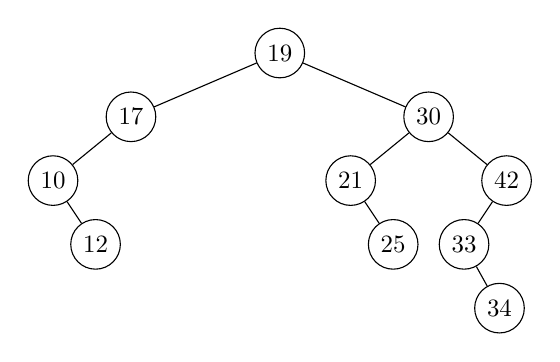
\begin{tikzpicture}[
    level distance=0.9cm,
    every node/.style={circle,draw,minimum size=7mm,inner sep=1pt},
    level 1/.style={sibling distance=4.2cm},
    level 2/.style={sibling distance=2.2cm},
    level 3/.style={sibling distance=1.2cm},
    level 4/.style={sibling distance=1cm},
    scale=0.9, transform shape
]
\node {19}
  child { node {17}
    child { node {10}
      child[missing]
      child { node {12} } }
    child[missing] }
  child { node {30}
    child { node {21}
      child[missing]
      child { node {25} } }
    child { node {42}
      child { node {33}
        child[missing]
        child { node {34} } }
      child[missing] } };
\end{tikzpicture}}

\begin{document}
\maketitle

\section{Bináris keresőfa}

\begin{frame}{Bináris keresőfa}
\begin{columns}
\begin{column}{0.58\linewidth}
\begin{itemize}
    \item Minden csúcs kulcsához képest a bal részfa kulcsai kisebbek.
    \item A jobb részfa kulcsai nagyobbak.
    \item A feltétel minden részfára és minden leszármazottra igaz.
\end{itemize}
\vspace{2mm}
Most különböző kulcsokkal dolgozunk.
\end{column}
\begin{column}{0.42\linewidth}
\scalebox{0.7}{\bstree}
\end{column}
\end{columns}
\end{frame}

\begin{frame}[t]{Mitől keresőfa?}
Nem elegendő csak a közvetlen gyerekeket ellenőrizni: a teljes bal részfában minden kulcsnak kisebbnek, a teljes jobb részfában minden kulcsnak nagyobbnak kell lennie.

\vspace{4mm}
\begin{itemize}
    \item Például a 21 bal részfájában csak 19 és 21 közötti kulcsok állhatnak.
    \item A 12 jobb részfájában 12-nél nagyobb, de 17-nél kisebb kulcsok állhatnak.
\end{itemize}
\end{frame}

\begin{frame}[t]{Bináris keresőfa építése}
Ha a kulcsokat ebben a sorrendben szúrjuk be:

\vspace{2mm}
\texttt{19, 17, 30, 10, 21, 12, 42, 25, 33, 34}

\vspace{1mm}
\begin{center}
\bstree
\end{center}

Tehát a fa alakja a beszúrási sorrendtől függ.
\end{frame}

\begin{frame}[t]{Feladat: építsünk keresőfát!}
Szúrjuk be ebben a sorrendben a következő kulcsokat, és hasonlítsuk össze a kapott fa magasságát az előző példáéval:

\vspace{4mm}
\texttt{25, 10, 34, 17, 42, 12, 30, 21, 33, 19}

\vspace{4mm}
Mi történik, ha a bemenet már rendezett?

\vspace{4mm}
\texttt{10, 12, 17, 19, 21, 25, 30, 33, 34, 42}
\end{frame}

\begin{frame}[t]{Inorder bejárás}
Bináris keresőfában az inorder bejárás a kulcsokat növekvő sorrendben adja meg.

\vspace{3mm}
\begin{columns}
\begin{column}{0.45\linewidth}
\bstree
\end{column}
\begin{column}{0.55\linewidth}
\texttt{10, 12, 17, 19, 21, 25, 30, 33, 34, 42}
\end{column}
\end{columns}
\end{frame}

\begin{frame}[t]{Fa rekonstruálása bejárásból}
Keresőfa esetén a preorder vagy postorder bejárásból is rekonstruálható az alak:
\begin{itemize}
    \item Preorder: az első kulcs a gyökér.
    \item Postorder: az utolsó kulcs a gyökér.
    \item A gyökérnél kisebb kulcsok a bal, nagyobbak a jobb részfába kerülnek; ezt rekurzívan ismételjük.
\end{itemize}

\vspace{3mm}
\textbf{Feladat:} rekonstruáljuk a fát a következő sorozatból:

\texttt{Preorder: 2, 1, 6, 3, 5, 8, 7, 9}
\end{frame}

\section{Alapműveletek}

\begin{frame}{Műveletek a keresőfán}
\begin{itemize}
    \item \texttt{search(t, k)}: a $k$ kulcsú csúcs megkeresése
    \item \texttt{insert(t, k)}: új kulcs beszúrása
    \item \texttt{min(t)}: a minimális kulcsú csúcs
    \item \texttt{remMin(t)}: a minimális csúcs eltávolítása
    \item \texttt{del(t, k)}: a $k$ kulcsú csúcs törlése
\end{itemize}

\vspace{3mm}
Mindegyik művelet költsége $\Ord(h)$, ahol $h$ a fa magassága. Kiegyensúlyozatlan fa esetén $h$ akár $n-1$ is lehet.
\end{frame}

\begin{frame}[t]{Keresés}
\begin{columns}
\begin{column}{0.58\linewidth}
Hasonlítsuk össze a keresett kulcsot az aktuális csúcs kulcsával:
\begin{itemize}
    \item Ha megegyezik, megtaláltuk.
    \item Ha kisebb, a bal részfában folytatjuk.
    \item Ha nagyobb, a jobb részfában folytatjuk.
    \item Üres részfához érve a kulcs nincs a fában.
\end{itemize}

\vspace{3mm}
\textbf{Példa:} 25 keresése: \texttt{19 $\to$ 30 $\to$ 21 $\to$ 25}.
\textbf{Feladat:} milyen útvonalon keressük a 23-at?
\end{column}
\begin{column}{0.42\linewidth}
\scalebox{0.6}{\bstree}
\end{column}
\end{columns}
\end{frame}

\begin{frame}[t]{Keresés rekurzívan}
\setlength{\stukiwidth}{14cm}
\begin{stukibox*}{search(t : Node*; k : $\mathbb{Z}$) : Node*}
\begin{IF}[20]{2}{\stm{t = \emptyset \textrm{ or } t \to key = k}}
    \stm{return\;t}
\ELSE
    \begin{IF}[50]{1}{\stm{k < t \to key}}
        \stm{return\;search(t \to left, k)}
    \ELSE
        \stm{return\;search(t \to right, k)}
    \end{IF}
\end{IF}
\end{stukibox*}

\vspace{3mm}
Az iteratív változat ugyanezt az útvonalat egy ciklusban járja be.
\end{frame}

\begin{frame}[t]{Beszúrás}
\begin{columns}
\begin{column}{0.58\linewidth}
\small
Az új kulcs helyét keresés közben találjuk meg: az első olyan üres gyerekpointerhez kerül, ahol a keresés megáll.

\vspace{2mm}
\begin{itemize}
    \item A beszúrás megőrzi a keresőfa tulajdonságát.
    \item Különböző kulcsokat feltételezünk; ismétlődő kulcs beszúrásakor a meglévő csúcsot megtartjuk.
    \item A keresés és a beszúrás ugyanannyi lépésű: $\Ord(h)$.
\end{itemize}

\vspace{2mm}
\textbf{Feladat:} szúrjuk be a 32-t a példafába. Melyik csúcs bal gyereke lesz?
\end{column}
\begin{column}{0.42\linewidth}
\scalebox{0.6}{\bstree}
\end{column}
\end{columns}
\end{frame}

\begin{frame}[t]{Törlés esetei}
\begin{columns}
\begin{column}{0.58\linewidth}
\small
\begin{enumerate}
    \item \textbf{Levél:} egyszerűen eltávolítjuk.
    \item \textbf{Egy gyerek:} a szülő pointerét a törlendő csúcs gyerekére állítjuk.
    \item \textbf{Két gyerek:} a csúcs kulcsát a jobb részfa minimumára cseréljük, majd ezt a minimumot töröljük.
\end{enumerate}

\vspace{3mm}
\textbf{Példa a fán:} töröljük rendre a 12-t (levél), a 42-t (egy gyerek), majd a 30-at (két gyerek).
\end{column}
\begin{column}{0.42\linewidth}
\scalebox{0.6}{\bstree}
\end{column}
\end{columns}
\end{frame}

\begin{frame}[t]{Minimum és a minimum eltávolítása}
\begin{columns}
\begin{column}{0.58\linewidth}
\small
Keresőfa minimuma: induljunk a gyökértől, és menjünk mindig balra, amíg lehet.

\vspace{2mm}
\begin{itemize}
    \item A minimum csúcsnak nincs bal gyereke.
    \item Eltávolításkor a csúcs jobb gyereke kerül a helyére.
    \item A maximum hasonlóan, mindig jobbra lépkedve kereshető meg.
\end{itemize}

\vspace{2mm}
\textbf{Feladat:} mi a minimum a példafában, és mi kerül a helyére az eltávolítása után?
\end{column}
\begin{column}{0.42\linewidth}
\scalebox{0.6}{\bstree}
\end{column}
\end{columns}
\end{frame}

\section{Inorder rákövetkező}

\begin{frame}[t]{Inorder rákövetkező}
\begin{columns}
\begin{column}{0.58\linewidth}
\texttt{inorder\_next(p)} a $p$ utáni csúcsot adja az inorder bejárásban. Szülőpointert is feltételezünk.

\vspace{3mm}
\begin{itemize}
    \item Ha van jobb részfája: annak minimuma a rákövetkező.
    \item Ha nincs jobb részfája: felfelé haladunk, amíg egy olyan szülőhöz érünk, ahonnan bal gyerekként jöttünk.
    \item Ha ilyen szülő nincs, $p$ volt az utolsó elem.
\end{itemize}
\end{column}
\begin{column}{0.42\linewidth}
\end{column}
\end{columns}
\end{frame}

\begin{frame}[t]{Feladat: rákövetkező}
\begin{center}
\bstree
\end{center}

\vspace{2mm}
Határozzuk meg a következő csúcsok inorder rákövetkezőjét:

\texttt{12, 21, 25, 30, 34, 42}
\end{frame}

\begin{frame}[t]{Keresőfa-tulajdonság ellenőrzése}
Ötlet: járjuk be a fát inorder sorrendben, és ellenőrizzük, hogy a kulcsok szigorúan növekvőek-e.

\vspace{3mm}
\begin{itemize}
    \item Szülőpointerrel a bejárás iteratívan megvalósítható az \texttt{inorder\_next} művelettel.
    \item Ha bármelyik kulcs nem nagyobb az előzőnél, a fa nem keresőfa.
    \item A bejárás összköltsége $\Ord(n)$.
\end{itemize}
\end{frame}

\begin{frame}[t]{Szorgalmi feladat}
Írjunk algoritmust, amely egy bináris keresőfában megkeresi a legnagyobb, $k$-nál kisebb kulcsot. Ha nincs ilyen kulcs, adjon vissza NULL-t.
\end{frame}

\end{document}
